\documentclass[12pt, a4paper]{article}

\usepackage[utf8]{inputenc}
\usepackage[russian]{babel}
\usepackage{geometry}
\usepackage{mathtools}
\usepackage{verbatim}
\usepackage{indentfirst}
\usepackage{caption}
\usepackage{subcaption}
\usepackage{import}
\usepackage{xifthen}
\usepackage{pdfpages}
\usepackage{transparent}
\usepackage{graphicx}
\usepackage{caption}
\usepackage{hyperref}
\usepackage{float}

\newcommand{\norm}[1]{\lVert #1 \rVert}
\newcommand{\abs}[1]{\lvert #1 \rvert}
\usepackage[oglav,spisok,boldsect,eqwhole,figwhole,hyperref,hyperprint,remarks,greekit]{./style/fn2kursstyle}

\graphicspath{{./style/}{./figures/}}

\frenchspacing

\title{Решение задач интерполирования}
\lab{4}
\author{М.\,А.~Каган}
\creator{И.\,А.~Яковлев}
\supervisor{}
\group{ФН2-51Б}
\date{2024}

\begin{document}
	\maketitle
	\tableofcontents
	
	\newpage
	

	
	\section-{Контрольные вопросы}
	
	\begin{enumerate}
	\item \textbf{Определите количество арифметических операций, требуемое для интерполирования функции в некоторой точке многочленом Лагранжа (включая построение самого многочлена) на сетке с числом узлов, равным n.}
	
	\vspace*{0.2cm}
	
	\textit{\textbf{Ответ:}}
	
	Для построения интерполяционного многочлена в форме Ньютона, необходимо посчитать следующую таблицу разделенных разностей:
	\begin{figure}[ht]
		\centering
		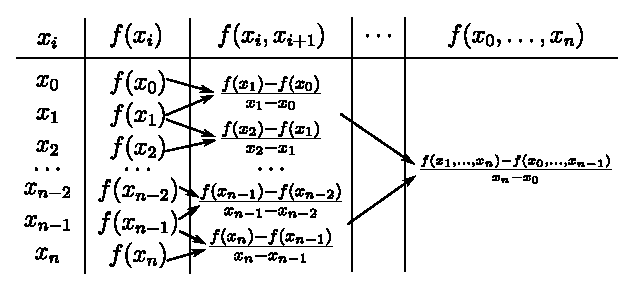
\includegraphics[scale=1.35]{таблица1.eps}
	\end{figure}
	
	В каждом последующем столбце количество строк уменьшается на одну, поскольку, чтобы посчитать значение  $f(x_i, \ldots, x_{i+k})$ с учетом того, что все необходимые коэффициенты известны, необходимо совершить одну операцию деления. Таким образом, нужно произвести $\sfrac{n(n-1)}{2} - n$ операций.
	
	Многочлен в форме Ньютона можно записать в виде:
	\[
	L_n(x) = f(x_0) + (x - x_0)f(x_1) + \ldots + (x - x_0)\ldots (x - x_n)f(x_n). 
	\]
	Точка $\tilde{x}$ --- точка, в которой необходимо вычислить значение функции $L_n(x)$. Так как все разделенные разности известны, остается вычислить множители:
	 \[
	 f(x_0,x_1, \ldots,x_{k+1})\prod\limits_{j = 0}^{k}(\tilde{x} - x_j)
	 \]
	где $k = 0, \ldots, n-1$. Если сохранять промежуточные вычисления $\prod\limits_{j = 0}^{k}(\tilde{x} - x_j)$, то количество операций умножения равняется $n$. 
	
	Таким образом общее количество необходимых операций: $\sfrac{n(n-1)}{2}$
	
	\item \textbf{Определите количество арифметических операций, требуемое для интерполирования функции в некоторой точке кубическим сплайном (включая затраты на вычисление коэффициентов сплайна) на сетке с числом узлов, равным n.}
	\vspace*{0.2cm}
	
	\textit{\textbf{Ответ:}}
	
	Пусть имеется $n$ штук узлов $\{ x_i\}_{i=1}^n$, на отрезках $[x_{i-1}, \, x_i]$ кубический сплайн задается функцией
$$
S(x) = a_i + b_i h_i + c_i h_i^2 + d_i h_i^3,
$$
где $h_i = x_i - x_{i- 1}$. Дополнив условиями непрерывности первых и вторых производных $S(x)$, получим систему
\begin{equation*}
	\begin{cases}
		c_1 = 0, \\
		c_{i - 1} h_{i -1} + 2 (h_i + h_{i-1}) c_i + c_{i+1} h_i = 3 (g_i - g_{i -1}), \\
		c_{n+1} = 0,
	\end{cases}
	\quad i = 2, 3, \dotsb, n,
\end{equation*}
где $g_i = \frac 1 h_i (f_i - f_{i - 1}), \, f_i = S(x_i)$. Тогда на вычисление коэффициентов $h$ и $g$ будет потрачено $2(n -1)$ операций, на вычисление $2(h_i + h_{i-1})$ и $3 (g_i - g_{i -1})$ будет потрачено $2(n - 2)$ операций, для вычисления коэффициентов $c_i$ необходимо будет использовать метод прогонки для системы размером $n - 1$, на что уйдет $5(n - 1) - 4$ операций. Для нахождения $b_i = g_i - \frac 1 3 (c_{i + 1} + 2 c_i) h_i$ и $d_i = \frac{1}{3 h_i} (c_{i + 1} - c_i)$ потребуется $5 (n - 1)$ операций, итого $O(13n)$ операций.

	\item \textbf{Функция $f(x) = e ^ x$ интерполируется многочленом Лагранжа на отрезке $[0, 2]$ на равномерной сетке с шагом $h=0.2$.Оцените ошибку экстраполяции в точке $x = 2.2$, построив многочлен Лагранжа и подставив в него это значение, а также по формуле для погрешности экстраполяции.}
	\vspace*{0.2cm}

	\textit{\textbf{Ответ:}}
	
	Погрешность с помощью прямых вычислений: $1.59 \cdot 10^{-7}$.
	
	Погрешность с помощью формулы:
	\[
	\abs{f(2.2) - L_n(2.2)} \le \dfrac{M_{n+1}}{(n+1)!}\abs{\omega(2.2)} \approx 1.85 \cdot 10^{-7},
	\]
	где $M_{n+1} = \norm{f^{(n+1)}(x)}_C$ и $\omega(x) = \prod\limits_{k=0}^{n}(x - x_k)$
	
	\item \textbf{Выпишите уравнения для параметров кубического сплайна, если в узлах $x_0$ и $x_n$ помимо значений функции $y_0$ и $y_n$ заданы первые производные $y'(x_0)$ и $y'(x_n)$.}
	
	\vspace*{0.2cm}
	
	\textit{\textbf{Ответ:}}

	На отрезках $[x_{i-1}, \, x_i]$ кубический сплайн задается функцией
	$$
	S(x_i) = a_i + b_i h_i + c_i h_i^2 + d_i h_i^3,
	$$
	где $h_i = x_i - x_{i- 1}$, $a_i = y_{i-1} = S(x_{i - 1})$. Первая и вторая производные функции $S(x_i)$:
	\begin{gather}
		S'(x_i) = b_i + 2 c_i h_i + 3 d_i h_i^2, \\
		S''(x_i) = 2 c_i + 6 d_i h_i.
	\end{gather}
	Необходимо ввести условие непрерывности производных на границах. Если принять $(x_i - 0) \in [x_{i-1}, \, x_i], \, (x_i + 0) \in [x_i, \, x_{i + 1}] $, то используя (1)-(2), получим 
	\begin{equation*}
		\begin{cases}
			b_i + 2 c_i h_i + 3 d_i h_i^2 = b_{i + 1}, \\
			2 c_i + 6 d_i h_i = 2 c_{i + 1}
		\end{cases}
		\quad i = \overline{1, n}.
	\end{equation*}
	Из второго уравнения системы выразим $d_i = \frac 1 {3h_i} (c_{i + 1} - c_i)$. Следующим шагом будет выражение $b_i$: 
	\[
	S(x_i) = y_i = y_{i -1} + b_i h_i + c_i h_i^2 + d_i h_i^3 \implies b_i = \frac 1 h_i (y_i - y_{i - 1}) - c_i h_i - d_i h_i ^2,
	\]
	положив $g_i = \frac{y_i - y_{i - 1}}{h_i}$, получим
	\[
	b_i = g_i - \frac{(c_{i + 1}+ 2 c_i)h_i}{3}, \quad i = \overline{1, n}.
	\]
	Подставив $b_i$ и $d_i$ в (1) и сместив индексацию $i \rightarrow i - 1$, получим
	\[
	h_{i-1} c_{i-1} + 2 (h_{i -1} + h_i) c_i + h_i c_{i + 1} = 3(g_i - g_{i -1}), \quad i = \overline{2,n}.
	\]
	Имем $n-1$ уравнение, $n+1$ неизвестных $\{c_i \}_{i=1}^{n+1}$. Добавим два уравнения исходя из условий
	\[
	S'(x_0) = y'(x_0), \quad S'(x_n) = y'(x_n),
	\]
	или 
	\[
	b_1 = y'(x_0), \quad b_n + 2 c_n h_n + 3 d_n h_n^2 = y'(x_n).
	\]
	Приводим к более простому виду:
	\begin{gather*}
		g_1 - \frac{(c_{2}+ 2 c_1)h_1}{3} = y'(x_0), \, \implies 2c_1 h_1 + c_2 h_1 = 3(g_1 - y'(x_0)).
	\end{gather*}
	Приводим второе уравнение к более простому виду. Запишем
	\[
		b_i + c_i h_i + d_i h_i^2 = g_i,
	\]
	при $n$
	\[
	b_n + c_n h_n + d_n h_n^2 = g_n,
	\]
	вычтем условие на правой границе
	\[
	c_n h_n + 2 d_n h_n^2 = y'(x_n) - g_n, \, \implies c_n h_n + 2 \frac{c_{n+1} - c_n}{3} h_n = y'(x_n) - g_n,
	\]
	откуда
	\[
	c_n h_n + 2 c_{n+1} h_n = 3(y'(x_n) - g_n).
	\]
	Итоговая система имеет вид:
	\begin{equation*}
		\begin{cases}
			2c_1 h_1 + c_2 h_1 = 3(g_1 - y'(x_0)), \\
			h_{i-1} c_{i-1} + 2 (h_{i -1} + h_i) c_i + h_i c_{i + 1} = 3(g_i - g_{i -1}), \quad i = \overline{2,n}, \\
			c_n h_n + 2 c_{n+1} h_n = 3(y'(x_n) - g_n).
		\end{cases}
	\end{equation*}
	
	\item \textbf{Каковы достоинства и недостатки сплайн-интерполяции и интерполяции многочленом Лагранжа?}
	\vspace*{0.2cm}
	
	\textit{\textbf{Ответ:}}
	
	\textbf{Интерполяция Лагранжа.}
	
	Достоинства:
	\begin{enumerate}
		\item Простота реализации;
		\item Высокая точность при сходимости;
		\item Есть возможность брать производную высшего порядка.
		\item Высокая точность интерполяции на малых отрезках.
	\end{enumerate}
	
	Недостатки:
	\begin{enumerate}
		\item Высокая алгоритмическая сложность построения (относительно сплайна);
		\item Высокая алгоритмическая сложность добавления узлов (относительно сплайна);
		\item Чувствительность к выбору сетки, в частности от этого может зависеть сходимость последовательности многочленов к функции (теоремы Фабера и Марцинкевича);
		\item Чувствительность к гладкости функции, например, по теореме Бернштейна на отрезке $[-1; 1]$ на равномерной сетке полиномы не сходятся к $\abs{x}$ во всех точках, кроме $\{-1, 0, 1\}$.
		 
	\end{enumerate}
	
	\textbf{Сплайн интерполяция.}
	
	Достоинства:
	\begin{enumerate}
		\item Высокая скорость построения интерполирующей функции;
		\item Высокая скорость добавления узлов;
		\item Стабильность вычислений;
		\item Сходимость на равномерной сетке;
		\item Сходимость первой и второй производной у сплайнов третьего порядка;
		\item Локальность интерполяции и гибкость в выборе порядка многочлена интерполяции.
	\end{enumerate}
	
	Недостатки:
	\begin{enumerate}
		\item Низкая скорость сходимости (относительно интерполяции Лагранжа);
		\item Сложность реализации, в частности для построения сплайнов разной степени на произвольных участках;
		\item Невозможность нахождения производных высшего порядка.
		\item Существование точек перегиба у сплайнов низкого порядка, из-за чего могут возникнуть проблемы при численном поиске производной: несовпадение знака производной, несуществующие нули у второй производной и т.д.
	\end{enumerate}
	
	\item \textbf{Какие свойства полиномов Чебышева и чебышевских сеток Вам известны?}
	\vspace*{0.2cm}
	
	\textit{\textbf{Ответ:}}

	\textbf{Основные свойства:}
	\begin{enumerate}
		\item Полиномы Чебышева $T_n(x)$ определяются рекурсивно:
		\[
		T_0(x) = 1, \, T_1(x) = x, \, T_{n+ 1}(x) = 2x T_n(x) - T_{n - 1}(x),
		\]
		или через тригонометрическую функцию
		\[
		T_n(x) = \cos (n \arccos x), \quad \abs{x} \le 1.
		\]
		\item Корни полинома $T_n(x)$ находятся на отрезке $[-1,\,1]$	и равны
		\[
		x_k = \cos \left(\frac{\pi (2k - 1)}{2n}\right), \quad k = \overline{1,n}.
		\]
		\item На отрезке $[-1, \, 1]$ значения $T_n(x)$ колеблются между $-1$ и $1$, достигая экстремумов в точках
		\[
		x_k = \cos \left( \frac{k \pi}{n}\right), \quad k = \overline{1,n}.
		\]
		\item Полиномы Чебышева минимизируют максимальное отклонение от нуля среди всех полиномов степени $n$ на отрезке $[-1, \, 1]$.
	\end{enumerate}
	\end{enumerate}
	



	
\end{document}